\chapter{Machine Learning Modelle}
In dieser Arbeit wird die Device-Based Indoor-Lokalisation auf Basis von Sensorwerten untersucht.
Der Ansatz ist inspiriert von dem Orientierungssinn von Mensch und Tier.
Dabei werden diskrete Standorte unterschieden, sowie ob eine Anomalie entdeckt wurde,
d. h. ob das Modell sich an einem unbekannten Standort oder auf einem unbekannten Pfad befindet.
\newline
\newline
Abbildung \ref{fig:model_idea} zeigt die Architektur des verfolgten Ansatzes.
Zunächst werden aus den Sensorwerten Features extrahiert.
Die resultierende Feature-Menge wird dann von dem ML-Modell genutzt, um den Standort zu klassifizieren.
Zuletzt wird auf Basis historischer Daten und dem Klassifizierungsergebnis von einem weiteren ML-Modell zur Anomalieerkennung bestimmt, ob eine Anomalie vorliegt.
Im Vergleich zur Architektur von Mian \cite{naveedThesis} können die Klassifizierungsergebnisse bei der Feature-Extrahierung weiter verarbeitet werden.
\begin{figure}[h!]
    \centering
    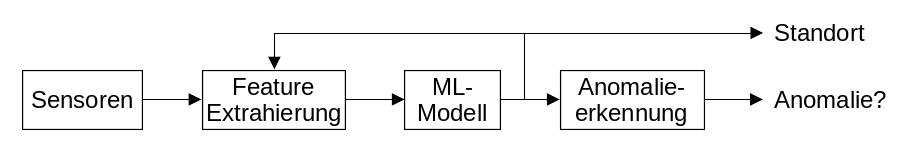
\includegraphics[width=\linewidth]{images/model_idea.png}
    \caption{Architektur des verfolgten Ansatzes.}
    \label{fig:model_idea}
\end{figure}
\newline
In dieser Arbeit werden Entscheidungsbaum basierte Klassifizierer mit KNN verglichen, insbesondere den von Mian verwendeten Ansatz mit FFNN.
Entscheidungsbäume sind deutlich effizienter in der Ausführungszeit als KNN \cite{dymelThesis},
allerdings sind sie in ihrer Generalisierungsfähigkeit durch die berechneten Features begrenzt,
wohingegen KNN komplexe Features selbst erlernen können.

\section{Standortenkodierung}
Als Standort wird ein einzigartiger diskreter Ort im Indoor-Szenario bezeichnet.
Bei der Klassifizierung können Standorte auf verschiedenen Arten im ML-Modell enkodiert werden.
Mian enkodierte die Pfade zwischen den Standorten, d. h. das Klassifizierungsergebnis ist der Pfad auf dem sich der Mikrocontroller befindet \cite{naveedThesis}.
\newline
\newline
Daneben wurden in dieser Arbeit noch zwei weitere Ansätze untersucht.
Im ersten Ansatz werden alle Punkte im Umkreis von bestimmten Punkten als Standorte definiert und alle restlichen als \textit{unbekannten Standort}.
Der zweite Ansatz kombiniert die beiden anderen Ansätze.
Zunächst werden, wie im ersten Ansatz, alle Punkte im Umkreis von bestimmten Punkten als Standorte definiert.
Dann werden die übrigen Punkte, also die Pfade zwischen zwei Standorten, als Standorte definiert.
\newline
\newline
Der Zusammenhang dieser Ansätze wird deutlich, wenn man eine Route als zyklischen Graphen betrachtet.
Einzigartige diskrete Punkte, die von interesse sind, bilden die Knoten und die Pfade zwischen diesen Punkten, die Kanten.
Mian's Ansatz nutzt nur die Kanten und folglich die anderen Ansätze jeweils die Knoten und die Knoten und Kanten.
\newline
\newline
Daraus wird die Komplexität und Genauigkeit dieser Ansätze deutlich.
Der Kantenansatz ist ein Kompromiss zwischen Genauigkeit und Komplexität.
Dabei bestimmt die Anzahl der zu klassifizierenden Standorte die Komplexität.
Zum einen ist gerade bei langen Pfaden eine geringe Auflösung im Vergleich zur Realposition zu erwarten,
d. h. es ist unklar, ob sich das Objekt am Anfang, Ende oder in dazwischen befindet.
Zum anderen werden in einem zyklischen Graphen mindestens so viele Standorte, wie beim Knotenansatz verwendet.
Der Knotenansatz benötigt am wenigsten Standorte zur Enkodierung ist aber außerhalb der Standorte sehr ungenau.
Aus einer Historie von vorherigen Standorten kann aber ein möglicher Pfad inferiert werden,
d. h. bei einer Gabelung können mehrere Pfade in Frage kommen.
Der kombinierte Ansatz bedarf enkodiert soviele Standorte wie beide Ansätze zusammen,
wodurch dieser Ansatz am komplexisten ist und am schlechtesten für große Routen skaliert.
Dafür ist die Auflösung des kombinierten Ansatzes so gut, wie eine diskrete Enkodierung es zulässt.
\newline
\newline
Ist in den aufgenommenen Trainingsdaten die Position des Objektes zum Zeitpunkt der Aufnahme der Sensorwerte bekannt,
so können die Standorte nach dem gewählten Enkodierungsansatz beliebig genau beschriftet werden.
Dies kann in einem Weiterverarbeitungsschritt nach der Aufnahme der Daten mit ein Karte von den Interessepunkten geschehen.
\newline
\newline
Bei der Evaluation in Kapitel \ref{sec:eval_anomalieerkennung} hat sich gezeigt, dass Anomalien besser erkannt werden können,
wenn die Auflösung des Enkodierungsansatzes hoch ist.
\section{Entscheidungswald}
\label{sec:model_dt}
Entscheidungsbaum basierte Klassifizierer sind sehr effizient und können trotzdem hohe Klassifizierungsgenauigkeiten bei hohen Fehlertoleranzen erreichen \cite{dymelThesis}.
Entscheidungswälder erhöhen die Klassifizierungsgenauigkeit während die Varianz reduziert wird, dafür wird aber der Speicherbedarf mit jedem Baum linear erhöht.
Der Klassifizierer soll zukünftig auf einem Mikrocontroller ausgeführt werden, d. h. die Größe des Entscheidungswaldes ist durch den Programmspeicher des Mikrocontrollers limitiert.
Zu dem Zeitpunkt, wo diese Arbeit verfasst wird, sind die Limitierungen des Mikrocontrollers noch nicht bekannt.
Für gewöhnlich ist der Programmspeicher aber auf wenige Kilo-Byte beschränkt \cite{dymelThesis}.
\newline
\newline
Als Ensemble-Methode wird \textit{RandomForest} benutzt, da dieser Entscheidungsbäume auf Basis von zufälligen Teilmengen der Feature-Menge konstruiert.
Dadurch ist eine erhöhte Toleranz gegenüber Fehlern, wie fehlerhafte Sensorwerte oder anderen Features zu erwarten.
\newpage
Um den Einfluss von verschiedenen Wald- und Baumgrößen auf die Fehlertoleranz und Klassifizierungsgenauigkeit hin zu untersuchen, werden verschiedene Größen
trainiert und auf den Testmengen evaluiert. Trotzdem wurden Dimensionen in einem Bereich gewählt, der für einen Mikrocontroller realistisch ist.
Es wurden jeweils Bäume und Wälder der Größe 8, 16, 32, und 64 untersucht.
\section{Feed Forward neuronales Netzwerk}
\label{sec:model_ffnn}
Für das KNN wird ein Feed Forward neuronales Netzwerk verwendet.
Das FFNN besteht aus drei bis sechs Schichten.
Alle Schichten, außer der letzten, verwenden ReLU als Aktivierungsfunktion.
Die letzte Schicht verwendet SoftMax.
\newline
\newline
Die Größe der Eingabeschicht ist abhängig von der Anzahl der verwendeten Features.
Die Features werden in einem Vorverarbeitungsschritt im Gegensatz zum Entscheidungswald normalisert.
Die Größe der Ausgabeschicht ist die Anzahl der verschieden diskreten Standorte, die unterschieden werden.
Je nach Konfiguration gibt es eins, zwei oder vier verdeckte Schichten, die jeweils 16, 32, 64 oder 128 Neuronen haben.
\newline
\newline
Die Standorte sind kategorische Daten, d. h. ihr Wert haben keine Aussage über die Beziehung der Standorte zueinander.
Aus diesem Grund werden sie kategorische Enkodiert, d. h. aus einem Wert $i$ aus $N$ möglichen Werten wird eine Liste der Größe $N$ generiert,
die überall 0 ist außer an der Stelle $i$, die 1 ist.
Folglich wird als Kostenfunktion \textit{kategorische Crossentropy} verwendet.
\newline
\newline
Als Lernalgorithmus wird Adam verwendet mit einer Batch-Größe von 50.
Trainiert wird über 75 Epochen.

\iffalse
\begin{itemize}
    \item Braucht man mehr Neuronen/Hidden Layer mit steigender Ort Anzahl?
\end{itemize}
\fi
\section{Training der ML-Modelle}
\label{sec:model_training}
Typischerweise haben weder Entscheidungsbaum basierte Klassifizierer noch FFNNs Rückwärtskanten.
Neuronale Netze mit Rückwärtskanten werden als \textit{rekurrente Netze} (RNN) bezeichnet.
Abbildung \ref{fig:model_idea} zeigt, dass die Rückwärtskante genutzt wird, um das Klassifizierungsergebnis,
also den vorherigen Standort, bei der Feature-Extrahierung zu nutzen.
Das Klassifizierungsergebnis ist aber nicht immer korrekt, wodurch fehlerhafte Features im Zusammenhang
mit dem Klassifizierungsergebnis als Eingabe in das ML-Modell verwendet werden können.
Damit das ML-Modell lernt mit diesem Fehler umzugehen, ist es notwendig, dass das ML-Modell Trainingsbeispiele mit
Features auf Basis eigener Klassifizierungsbeispiele zur Verfügung hat.
\newline
\newline
Abbildung \ref{fig:training_explained} illustriert den Trainingsablauf.
Die simulierten Daten der aufgenommenen Routen sind unterteilt in Partitionen basierend auf deren Zyklusbeschriftung,
damit in jeder Partition alle Standorte vorhanden sind.
Der Zyklus ist ein Umlauf einer Route, bevor sie wiederholt wird.
Insgesamt besteht die Datenmenge aus 20 Zyklen.
Die ersten fünf Zyklen werden zum \glqq Aufwärmen \grqq\ verwendet,
d. h. das ML-Modell wird mit korrekt beschrifteten Daten trainiert, welche es nicht selbst beschriftet hat.
In den folgenden zehn Zyklen werden weitere Partitionen zur Trainingsmenge hinzugefügt, die mit quadratisch steigendem Anteil vom ML-Modell selbst beschriftet sind.
Zunächst werden 50\% der Partition $i$ vom ML-Modell beschriftet, bis beim 13. Zyklus schließlich 100\% beschriftet wird.
Die Elemente aus der Partition, die beschriftet werden sollen, sind zufällig, damit der Klassifizierungsfehler auf allen Teilstücken der Route gelernt werden kann.
\begin{figure}[h!]
    \centering
    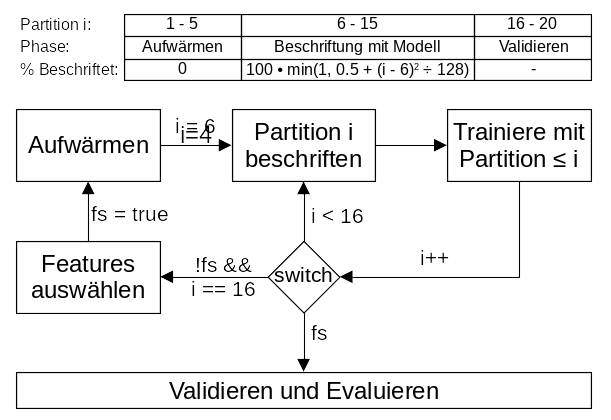
\includegraphics[width=\linewidth]{images/training_explained.png}
    \caption{Der Trainingsablauf des verfolgten Ansatzes.}
    \label{fig:training_explained}
\end{figure}
\newline
\newline
Die erste Trainingsphase ist abgeschlossen, nachdem das ML-Modell mit einer Trainingsmenge von 15 Zyklen trainiert wurde.
Anschließend wird einmalig eine Feature-Auswahl betrieben, in der insignifikante Features aus der Feature-Menge entfernt werden.
Features sind insignifikant, die eine geringe Wichtigkeit aufweisen (Kapitel \ref{sec:eval_feature_importance}).
Dies ermöglicht kleinere ML-Modelle zu verwenden und verringert die Dimensionen des Suchraumes, wodurch das Trainieren erleichtert wird.
Außerdem müssen Modelle individuell für verschiedene Einsatzgebiete trainiert werden, bei denen möglicherweise einige Sensoren bzw. Features nicht genutzt werden.
In Abbildung \ref{fig:training_explained} ist die Feature-Auswahl nur einmalig vorgesehen.
Denkbar wäre aber auch eine iterative Eliminierung der Features oder Optimierung durch ein evolutionären Algorithmus.
Anschließend wird das ML-Modell erneut auf den Partitionen trainiert, bis es validiert und evaluiert werden kann.
\newline
\newline
Die ML-Modelle ohne Rückwärtskante sind deutlich simpler.
Diese müssen nicht in Zyklen trainiert werden, sondern können direkt mit der vollständigen Trainingsmenge trainiert werden,
wodurch das Training deutlich effizienter ist.
\section{Klassifizierungsgenauigkeit der Anomalien}
\label{sec:eval_anomalieerkennung}
Bei der Anomalieerkennung werden Entscheidungswälder und FFNNs mit den besten ML-Modellen zur Standorterkennung trainiert und mit den drei Baseline-Modellen verglichen.
Tabelle \ref{tab:anomaly_detection_prediction_accuracy} zeigt die Klassifizierungsgenauigkeiten über die verschiedenen Standortkomplexitäten,
wobei die Klassifizierungsgenauigkeit $P(A)$ nochmal genauer aufgeschlüsselt ist in den Anteil der korrekten Klassifizierungen, wenn eine bzw. keine Anomalie vorlag.
Die trainierten FFNNs geben stets aus, dass keine Anomalie vorliegt.
Es ist unklar, warum die FFNNs sich so verhalten.
\begin{table}[h!]
    \hspace{-1cm}
    \begin{tabular}{ | l | c | c | c | c | c | c | c | c | }
        \hline
        Standorte & 9 & 16 & 17 & 25 & 32 & 48 & 52 & 102 \\\hline
        \multicolumn{9}{ | l |}{$P(A)$}\\\hline
        Entscheidungswald & 82,59\% & 81,19\% & 87,14\% & 84,91\% & 79,06\% & 83,47\% & 81,93\% & 76,00\% \\\hline
        FFNN & 77,88\% & 77,88\% & 77,88\% & 77,88\% & 77,88\% & 77,88\% & 77,88\% & 77,88\% \\\hline
        Topologie (DT) & 84,77\% & 30,57\% & 83,51\% & 79,76\% & 28,63\% & 24,97\% & 80,55\% & 29,47\% \\\hline
        Topologie (KNN) & 86,10\% & 52,17\% & 77,72\% & 79,30\% & 45,06\% & 41,92\% & 74,77\% & 43,55\% \\\hline
        \multicolumn{9}{ | l |}{Anteil korrekt klassifiziert, indem Anomalie vorlag}\\\hline
        Entscheidungswald & 34,86\% & 35,52\% & 52,58\% & 50,92\% & 32,21\% & 50,64\% & 23,21\% & 1,92\% \\\hline
        FFNN & 0,00\% & 0,00\% & 0,00\% & 0,00\% & 0,00\% & 0,00\% & 0,00\% & 0,00\% \\\hline
        \multicolumn{9}{ | l |}{Anteil korrekt klassifiziert, indem keine Anomalie vorlag}\\\hline
        Entscheidungswald & 96,14\% & 94,41\% & 97,05\% & 95,83\% & 92,48\% & 93,13\% & 98,96\% & 97,18\% \\\hline
        FFNN & 100,00\% & 100,00\% & 100,00\% & 100,00\% & 100,00\% & 100,00\% & 100,00\% & 100,00\% \\\hline
    \end{tabular}
    \caption{$P(A)$ über Standorte und Modelle zur Anomalieerkennung.}
    \label{tab:anomaly_detection_prediction_accuracy}
\end{table}
\newpage
Die Entscheidungswälder hingegen eignen sich besser für den Anomalieerkennungszweck.
Es werden zwischen 1,92\% und 52,58\% der Anomalien erkannt und zwischen 1,04\% und 7,52\% falsch als Anomalien erkannt.
Die Klassifizierungsgenauigkeit des Entscheidungswaldes zur Anomalieerkennung ist abhängig von der Klassifizierungsgenauigkeit zur Standorterkennung
und von der Standortkomplexität.
Je besser das Standorterkennungsmodell und je höher die Standortkomplexität, desto höher ist die Anomalieerkennungsrate.
Aus diesem Grund ist die Klassifizierungsgenauigkeit bei den Standortkomplexitäten, die mit der Kodierungsmethode mit Kanten und Knoten zusammenhängen,
geringer, als bei der Kodierungsmethode, bei der nur die Knoten kodiert werden.
\newline
\newline
Abbildung \ref{fig:true_vs_predicted_anomaly} zeigt einen Auscchnitt der Anomalietestmenge, worauf der Entscheidungswald der Standortkomplexität 17 angewendet wurde.
Die Anomalie wird nicht kontinuierlich erkannt und es werden auch fälschlicherweise Standorte als Anomalien klassifiziert.
Allerdings treten falsch-positive Ergebnisse nur vereinzelt auf, wohingegen bei einer Anomalie, sehr häufig eine Anomalie erkannt wird.
Die falsch-positiven Ergebnisse können somit durch Ausnutzen dieser Fluktuationen vermieden werden,
indem beispielweise ein Schwellenwert an Ausschlägen in einer bestimmten Zeit eingeführt wird.
\begin{figure}[h!]
    \centering
    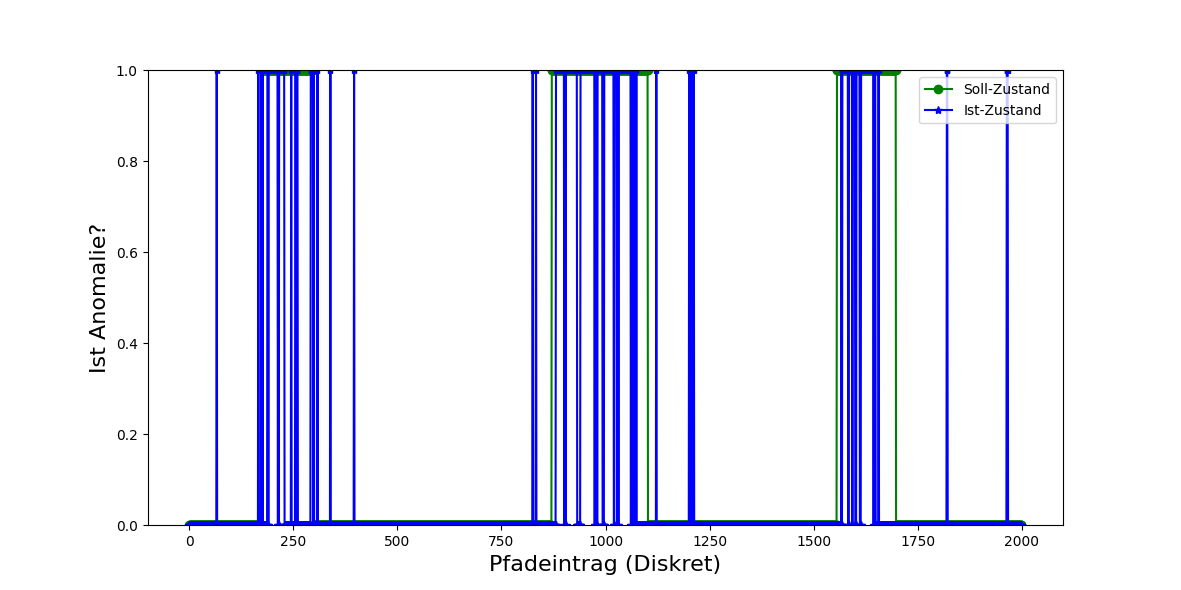
\includegraphics[width=\linewidth]{images/anomaly_true_vs_predicted.png}
    \caption{Ausschnitt der Klassifizierungsergebnisse auf der Anomalietestmenge mit dem Entscheidungswald der Standortkomplexität 17. }
    \label{fig:true_vs_predicted_anomaly}
\end{figure}

